% Created 2016-01-05 Tue 07:51
\documentclass[11pt]{article}
\usepackage[utf8]{inputenc}
\usepackage[T1]{fontenc}
\usepackage{fixltx2e}
\usepackage{graphicx}
\usepackage{grffile}
\usepackage{longtable}
\usepackage{wrapfig}
\usepackage{rotating}
\usepackage[normalem]{ulem}
\usepackage{amsmath}
\usepackage{textcomp}
\usepackage{amssymb}
\usepackage{capt-of}
\usepackage{hyperref}
\author{Chris Howe-Jones}
\date{15th December 2015}
\title{The Never Changing Face of Immutability}
\hypersetup{
 pdfauthor={Chris Howe-Jones},
 pdftitle={The Never Changing Face of Immutability},
 pdfkeywords={},
 pdfsubject={},
 pdfcreator={Emacs 24.5.1 (Org mode 8.3.2)},
 pdflang={English}}
\begin{document}

\maketitle

\section*{Warning!!}
\label{sec:orgheadline1}

\begin{itemize}
\item There will be a Lisp!
\item There will be Entomology!
\item There will be History!
\end{itemize}


\section*{The Never Changing Face of Immutability}
\label{sec:orgheadline29}

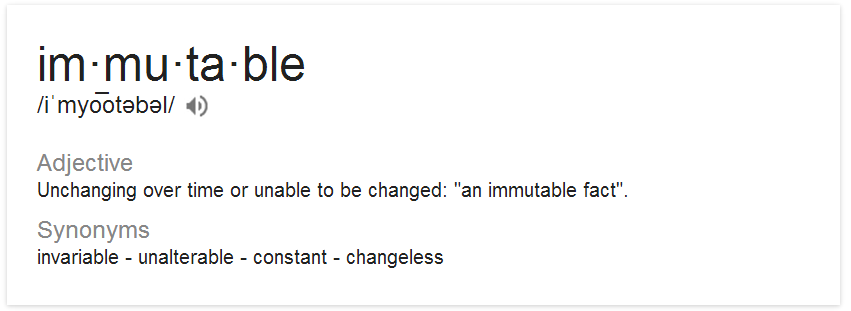
\includegraphics[width=.9\linewidth]{./immutable-defined.png}

\subsubsection*{Who am I?}
\label{sec:orgheadline2}

Name:      \texttt{Chris Howe-Jones}

Job Title: \texttt{Technical Navigator}

Twitter:   \texttt{@agile\_geek}

Github:    \texttt{github.com/chrishowejones}

Blog:      \texttt{chrishowejones.wordpress.com}

\subsubsection*{Credentials}
\label{sec:orgheadline3}

\begin{itemize}
\item 28 years of pushing data around
\item Procedural/OOP/FP
\item Architecture \& Design
\item RAD/Agile/Lean
\item CTO
\end{itemize}

\subsection*{History Lesson}
\label{sec:orgheadline4}

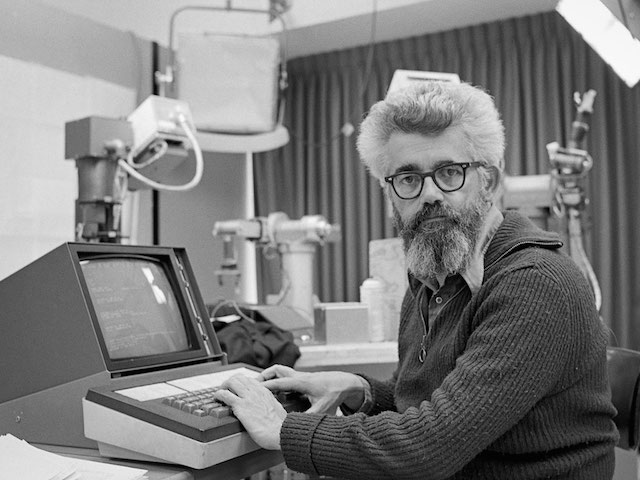
\includegraphics[width=.9\linewidth]{./John-McCarthy.jpg}

\subsection*{Once upon a time..}
\label{sec:orgheadline8}

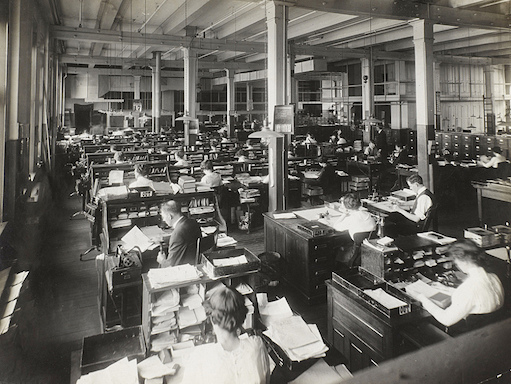
\includegraphics[width=.9\linewidth]{./book-keepers.jpg}

Book Keeping
\begin{itemize}
\item List of entries in a ledger
\end{itemize}
\begin{itemize}
\item No 'crossing out'!
\end{itemize}

\subsubsection*{Dawn of Computing}
\label{sec:orgheadline5}

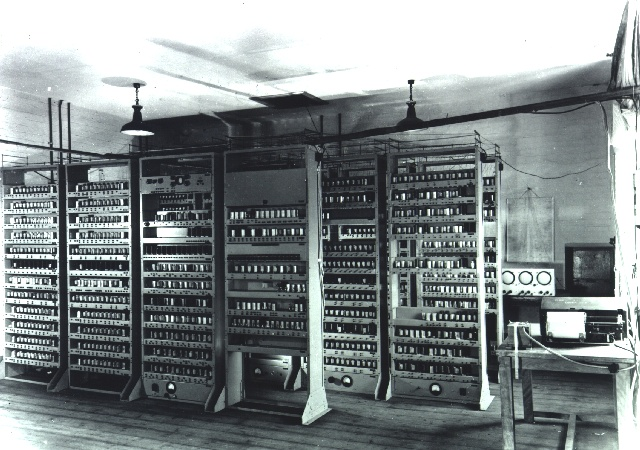
\includegraphics[width=.9\linewidth]{./EDSAC.jpg}

\begin{itemize}
\item Math
\item Transient storage
\end{itemize}

\subsubsection*{60's-90's}
\label{sec:orgheadline6}

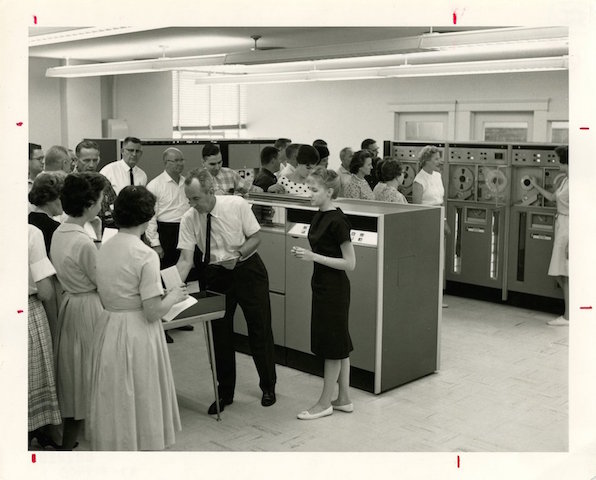
\includegraphics[width=.9\linewidth]{./1960s-computer.jpg}

\begin{itemize}
\item Spot the expense?
\end{itemize}
\begin{itemize}
\item Memory
\end{itemize}
\begin{itemize}
\item Tape
\end{itemize}
\begin{itemize}
\item Disk
\end{itemize}


\subsubsection*{21st Century}
\label{sec:orgheadline7}

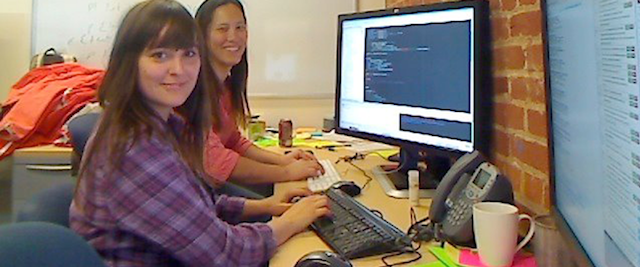
\includegraphics[width=.9\linewidth]{./pair-programming.png}

Spot the expense?
\begin{itemize}
\item Developers
\end{itemize}
Cheap resources: SSD/Disk, Memory, CPU


\subsection*{And..}
\label{sec:orgheadline11}


\includegraphics[width=.9\linewidth]{./fry-so.jpg}

\subsubsection*{In place computing}
\label{sec:orgheadline9}

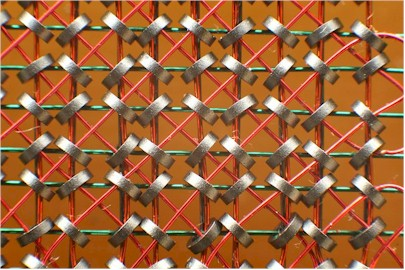
\includegraphics[width=.9\linewidth]{./core_memory.jpg}

\begin{itemize}
\item Update data in place
\end{itemize}
\begin{itemize}
\item Reuse expensive real estate
\end{itemize}

\subsubsection*{RDBMS}
\label{sec:orgheadline10}

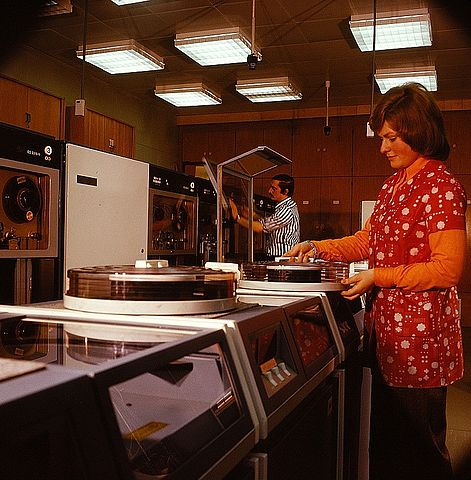
\includegraphics[width=.9\linewidth]{./disk-pack.jpg}

\begin{itemize}
\item Data updated
\end{itemize}
\begin{itemize}
\item Values overwritten
\end{itemize}
\begin{itemize}
\item Reuse memory and disk
\end{itemize}

\subsection*{Result?}
\label{sec:orgheadline16}

In place oriented programming (PLOP) relies on\ldots{}

\subsubsection*{Mutation}
\label{sec:orgheadline12}


\includegraphics[width=.9\linewidth]{./mutation.jpg}

\subsubsection*{Which leads to..}
\label{sec:orgheadline13}

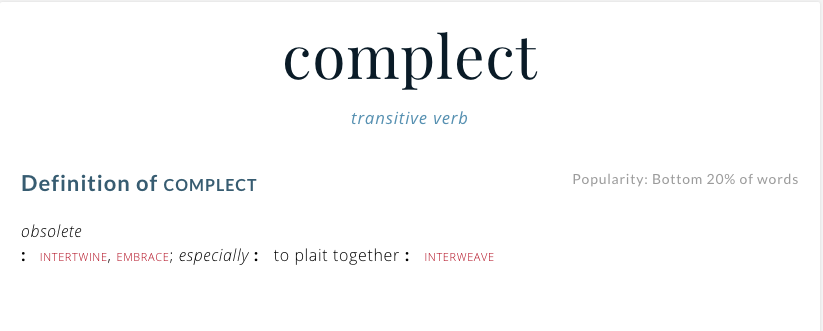
\includegraphics[width=.9\linewidth]{./complect.png}

\subsubsection*{Complect}
\label{sec:orgheadline14}

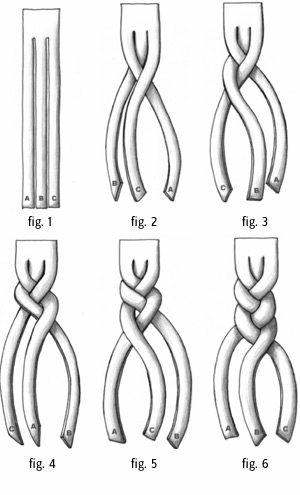
\includegraphics[width=.9\linewidth]{./plaiting.jpg}

\begin{itemize}
\item Complecting Identity \& Value
\end{itemize}
\begin{itemize}
\item Especially RDBMS, OOP
\end{itemize}
\begin{itemize}
\item Pessimistic concurrency strategies
\end{itemize}

\subsubsection*{What's changed?}
\label{sec:orgheadline15}
\url{./historical_cost_graph5.gif}

\begin{itemize}
\item Computing capacity has increased by a million fold!
\end{itemize}

\subsection*{Immutability (and values) to the rescue!}
\label{sec:orgheadline19}

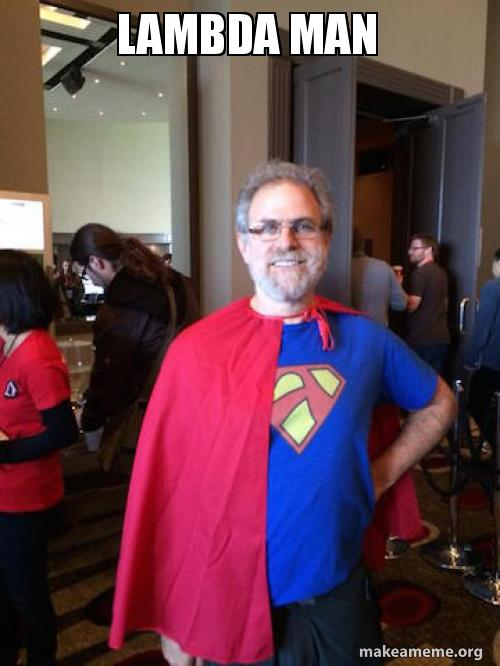
\includegraphics[width=.9\linewidth]{./lambda-man.jpg}

\subsubsection*{Values}
\label{sec:orgheadline17}


\includegraphics[width=.9\linewidth]{./values.jpeg}
\begin{itemize}
\item Values are generic
\item Values are easy to fabricate
\item Drives reuse
\item Values aggregate to values
\item Distributable
\end{itemize}

\subsubsection*{Isn't copying values inefficient?}
\label{sec:orgheadline18}

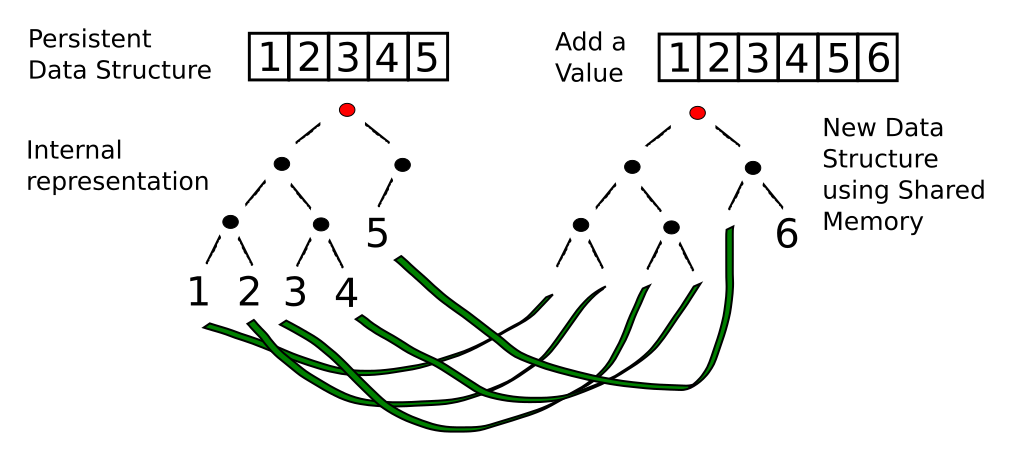
\includegraphics[width=.9\linewidth]{./clojure-persistent-data-structures-sharing.png}

\begin{itemize}
\item Structural sharing
\item For example in Clojure:
\begin{itemize}
\item persistent bit-partitioned vector trie
\item 32 node tries
\item Wide shallow trees
\end{itemize}
\end{itemize}

\subsection*{What does it look like?}
\label{sec:orgheadline22}

\begin{itemize}
\item Immutable by default
\item Explicit state change
\item Database as a value
\end{itemize}

\subsubsection*{ClojureScript on the client}
\label{sec:orgheadline20}

\begin{verbatim}
(def initial-state
  {:event {:event/name "" :event/speaker ""} :server-state nil})
\end{verbatim}
\begin{verbatim}
(defn- event-form
  [ui-channel {:keys [event/name event/speaker] :as event}]
  [:table.table
   [:tr
    [:td [:label "Event name:"]]
    [:td [:input {:type :text
                  :placeholder "Event name..."
                  :defaultValue event/name
                  :on-change (send-value! ui-channel m/->ChangeEventName)}]]]
   [:tr
    [:td [:label "Speaker:"]]
    [:td [:input {:type :text
                  :placeholder "Speaker..."
                  :defaultValue event/speaker
                  :on-change (send-value! ui-channel m/->ChangeEventSpeaker)}]]]
   [:tr
    [:td
     [:button.btn.btn-success
      {:on-click (send! ui-channel (m/->CreateEvent))}
      "Go"]]]])
\end{verbatim}

\begin{verbatim}
(defrecord ChangeEventName [name])

(defrecord ChangeEventSpeaker [speaker])

(defrecord CreateEvent [event])

(defrecord CreateEventResults [body])
\end{verbatim}
\begin{verbatim}
(extend-protocol Message
  m/ChangeEventName
  (process-message [{:keys [name]} app]
    (assoc-in app [:event :event/name] name)))
;; redacted for clarity ...

(extend-protocol EventSource
  m/CreateEvent
  (watch-channels [_ {:keys [event]
                      :as app}]
    #{(rest/create-event event)}))

(extend-protocol Message
  m/CreateEventResults
  (process-message [response app]
    (assoc app :server-state (-> response :body))))
\end{verbatim}

\subsubsection*{Efficiency}
\label{sec:orgheadline21}

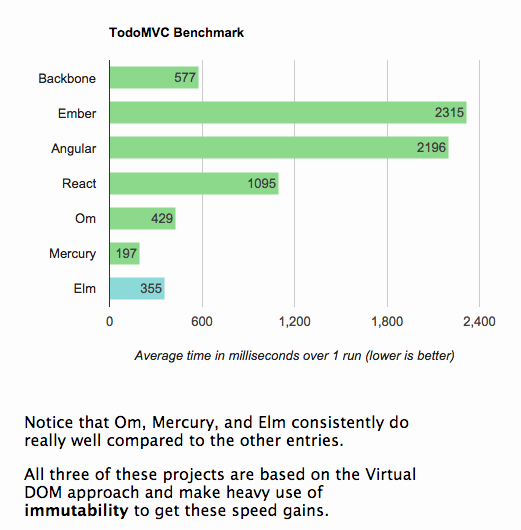
\includegraphics[width=.9\linewidth]{./todomvc-perf-comparison.png}

\subsection*{Clojure on the server}
\label{sec:orgheadline23}

\begin{verbatim}
(defn- handle-query
  [db-conn]
  (fn [{req-body :body-params}]
    {:body (case (:type req-body)
             :get-events (data/get-events db-conn)
             :create-event (data/create-entity db-conn (:txn-data req-body)))}))


(defn app [dbconn]
  (-> (routes
       (GET "/" [] home-page)
       (POST "/q" []
             (handle-query dbconn))
       (resources "/"))
      (wrap-restful-format :formats [:edn :transit-json])
      (rmd/wrap-defaults (-> rmd/site-defaults
                             (assoc-in [:security :anti-forgery] false)))))
\end{verbatim}

\subsection*{Datomic for Data}
\label{sec:orgheadline27}

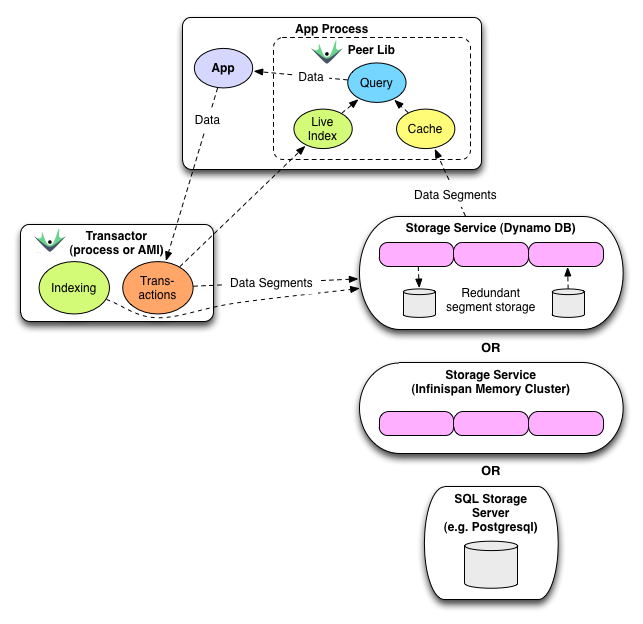
\includegraphics[width=.9\linewidth]{./datomic-architecture.png}

\begin{itemize}
\item App get's its own query, comms, memory- Each App is a peer
\end{itemize}

\subsubsection*{Database as a value}
\label{sec:orgheadline24}

\begin{center}
\begin{tabular}{llll}
Entity & Attribute & Value & Time\\
\hline
Fiona & likes & Ruby & 01/06/2015\\
Dave & likes & Haskell & 25/09/2015\\
Fiona & likes & Clojure & 15/12/2015\\
 &  &  & \\
\hline
 &  &  & \\
\end{tabular}
\end{center}

\begin{itemize}
\item Effectively DB is local
\item Datalog query language
\end{itemize}
\begin{verbatim}
[:find ?e :where [?e :likes “Clojure”]]
\end{verbatim}

\subsubsection*{Schema}
\label{sec:orgheadline25}

\begin{verbatim}
 ;;event
 {
  :db/id                 #db/id[:db.part/db]
  :db/ident              :event/name
  :db/cardinality        :db.cardinality/one
  :db/valueType          :db.type/string
  :db/unique             :db.unique/identity
  :db.install/_attribute :db.part/db
  }
 {
  :db/id                 #db/id[:db.part/db]
  :db/ident              :event/description
  :db/cardinality        :db.cardinality/one
  :db/valueType          :db.type/string
  :db.install/_attribute :db.part/db
  }
 {
  :db/id                 #db/id[:db.part/db]
  :db/ident              :event/location
  :db/cardinality        :db.cardinality/one
  :db/valueType          :db.type/ref
  :db.install/_attribute :db.part/db
  }
...
\end{verbatim}
\begin{verbatim}
;;location
 {
  :db/id                 #db/id[:db.part/db]
  :db/ident              :location/postCode
  :db/cardinality        :db.cardinality/one
  :db/valueType          :db.type/string
  :db.install/_attribute :db.part/db
  }
 {
  :db/id                 #db/id[:db.part/db]
  :db/ident              :location/description
  :db/cardinality        :db.cardinality/one
  :db/valueType          :db.type/string
  :db.install/_attribute :db.part/db
  }
...
\end{verbatim}
\subsubsection*{Persistence}
\label{sec:orgheadline26}

\begin{verbatim}
(defn create-entity
  "Takes transaction data and returns the resolved tempid"
  [conn tx-data]
  (let [had-id (contains? tx-data ":db/id")
        data-with-id (if had-id
                       tx-data
                       (assoc tx-data :db/id #db/id[:db.part/user -1000001]))
        tx @(d/transact conn [data-with-id])]
    (if had-id (tx-data ":db/id")
        (d/resolve-tempid (d/db conn) (:tempids tx)
                          (d/tempid :db.part/user -1000001)))))
\end{verbatim}
\begin{verbatim}
(defn get-events [db]
  (d/pull-many db [:*]
               (->> (d/q '{:find [?event-id]
                           :where [[?event-id :event/name]]}
                         db)
                    (map first))))
\end{verbatim}

\subsection*{Conclusion?}
\label{sec:orgheadline28}

\includegraphics[width=.9\linewidth]{./you-cant-step.jpg}
\begin{itemize}
\item Immutability simplifies
\item State as function call stack
\item Mostly pure functions
\begin{itemize}
\item Easier to test \& reason about
\end{itemize}
\item Time as first class concept
\item Easier to distribute
\end{itemize}

\section*{Resources}
\label{sec:orgheadline30}

\begin{itemize}
\item Rich Hickey talks -
\begin{itemize}
\item 'The Value of Values'
\item 'The Language of the System'
\item 'Simple Made Easy'
\item 'Clojure, Made Simple'
\item 'The Database as a Value'
\item 'The Language of Systems'
\end{itemize}
\item Moseley and Marks - Out of the Tar Pit
\item Kris Jenkins
\begin{itemize}
\item 'ClojureScript - Architecting for Scale' (Clojure eXchange 2015)
\end{itemize}
\end{itemize}
\end{document}
